
\chapter{Implementazione dei semafori nel modulo sistema}

\section{Descrittore di semaforo \emph{des$\_$sem}}
Il \textbf{descrittore di semaforo} è una struttura contenente le informazioni di un semaforo: un contatore (per ricordarci i gettoni presenti) e un puntatore alla lista dei processi in attesa del gettone. 	
\begin{verbatim}
	struct des_sem {
		int counter;
		des_proc *pointer;	
	};
\end{verbatim}
Le strutture dati sono poste nel modulo sistema, dunque sono inaccessibili all'utente se non invocando le primitive:
\begin{itemize}
	\item l'accesso è controllato (l'utente non può fare cose che non ci aspettiamo);
	\item si ha atomicità (non si pone la questione della mutua esclusione).
\end{itemize} 
\section{Array dei semafori \emph{array$\_$dess}} 
I semafori non vengono mai deallocati, quindi possiamo allocarli sequenzialmente in un'array.
\begin{verbatim}
	des_sem array_dess[MAX_SEM*2];
\end{verbatim}
\paragraph{Numero massimo di semafori} Creare un'array significa stabilire un numero massimo di semafori. La costante \emph{MAX$\_$SEM}, posta in \emph{include/costanti.h}
\begin{verbatim}
	#define MAX_SEM         1024UL
\end{verbatim}
indica il numero massimo di semafori per la modalità utente e per la modalità sistema. L'array \emph{array$\_$dess} è composto da $\text{MAX$\_$SEM}*2$ elementi:
\begin{itemize}
	\item la prima metà dell'array è riservata ai semafori in modalità utente;
	\item la seconda metà ai semafori in modalità sistema.
\end{itemize}
Chiaramente non possiamo permettere l'accesso alla seconda parte dell'array quando ci troviamo in modalità utente. 
\paragraph{Numero di semafori allocati} Con due variabili teniamo a mente il numero di semafori allocati nella prima e nella seconda parte dell'array:
\begin{verbatim}
	natl sem_allocati_utente = 0;
	natl sem_allocati_sistema = 0;
\end{verbatim}
Considerata l'allocazione sequenziale quanto memorizzato è sufficiente per trovare il primo semaforo non utilizzato.

%Non esiste una primitiva per distruggere un semaforo, la cosa sarebbe molto complessa.
\section{Primitiva per l'allocazione del semaforo}
\subsection{Funzione di utilità \emph{alloca$\_$sem}}
\small 
\begin{verbatim}
	natl alloca_sem() {
		int liv = liv_chiamante();
		natl i;
		if(liv == LIV_UTENTE) {
			if(sem_allocati_utente >= MAX_SEM)
			return 0xFFFFFFFF;
			i = sem_allocati_utente;
			sem_allocati_utente++;
		}
		else {
			if(sem_allocati_sistema >= MAX_SEM)
			return 0xFFFFFFFF;
			i = sem_allocati_sistema + MAX_SEM;
			sem_allocati_sistema++;
		}
		return i;
	}
\end{verbatim}
\normalsize 
\begin{itemize}	
	\item La funzione di utilità \emph{alloca$\_$sem} viene chiamata dalla primitiva \emph{sem$\_$ini}: essa restituisce l'indice del primo semaforo non utilizzato.
	\item Con la funzione di utilità \emph{liv$\_$chiamante} recuperiamo il livello di privilegio prima del lancio della primitiva. 
	\item Tengo conto del valore di \emph{MAX$\_$SEM}, e verifico se ho raggiunto il numero massimo di semafori possibili relativamente a una modalità. Se ciò avviene restituisco
	\begin{verbatim}
		return 0xFFFFFFFF;
	\end{verbatim}
	altrimenti restituisco l'indice del primo elemento array disponibile, e incremento la relativa variabile contatore. 
	\item Ricordarsi che la prima parte dell'array è dedicata alla modalità utente, mentre la seconda alla modalità sistema.
\end{itemize}
\subsection{Primitiva \emph{sem$\_$ini}}
\small 
\begin{verbatim}
	// parte "C++" della primitiva sem_ini
	extern "C" void c_sem_ini(int val) {
		natl i = alloca_sem();
		
		if(i != 0xFFFFFFFF)
		array_dess[i].counter = val;
		
		esecuzione->contesto[I_RAX] = i;
	}
\end{verbatim}
\normalsize 
%\begin{center}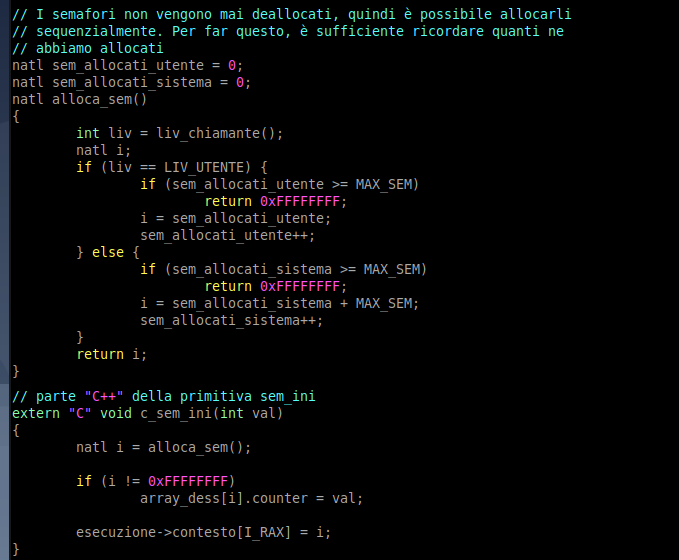
\includegraphics[scale=.8]{img/193.PNG}\end{center}
\begin{itemize}
	\item Per la creazione del semaforo utilizziamo la primitiva \emph{sem$\_$ini}. Il parametro di ingresso  \emph{val} contiene il numero di gettoni iniziali del semaforo.
	\item Con la funzione di utilità \emph{alloca$\_$sem} otteniamo l'indice del primo semaforo non utilizzato dell'array.
	\item Se la funzione non ha restituito il valore di errore manipolo il semaforo avente indice \emph{i}: imposto il \emph{counter} col valore del parametro di ingresso \emph{val} e restituisco \emph{i} aggiornando il contesto di \emph{esecuzione}.
	\begin{verbatim}
		esecuzione->contesto[I_RAX] = i;
	\end{verbatim}
\end{itemize}

\section{Primitive per la gestione dei semafori}

\subsection{Funzione di utilità \emph{sem$\_$valido}} 
\small
\begin{verbatim}
	bool sem_valido(natl sem) {
		int liv = liv_chiamante();
		return sem < sem_allocati_utente || (liv == LIV_SISTEMA && sem - MAX_SEM < sem_allocati_sistema);
	}
\end{verbatim}
\normalsize
%\begin{center}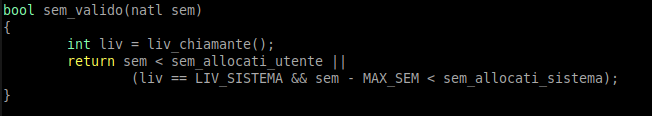
\includegraphics[scale=.9]{img/194.PNG}\end{center} 
\begin{itemize}
	\item Recupero il livello  di privilegio antecedente la chiamata della primitiva con la funzione di utilità \emph{liv$\_$chiamante}.
	\item Uso il valore restituito (posto in \emph{liv}) e il parametro di ingresso \emph{sem} (identificativo di un semaforo) per verificare se questo è valido.
	\begin{itemize}
		\item \textbf{Modalità utente}.
		
		Il semaforo è valido se \emph{sem} è minore del numero di semafori allocati in modalità utente (\emph{sem$\_$allocati$\_$utente}) (ci troviamo nella prima metà dell'array).
		\item \textbf{Modalità sistema}. 
		
		Il semaforo è valido se la differenza tra \emph{sem} e \emph{MAX$\_$SEM} è minore del numero di semafori allocati in modalità sistema (\emph{sem$\_$allocati$\_$sistema}, ci troviamo nella seconda parte dell'array). Dobbiamo anche verificare che il livello del chiamante sia di sistema.  
	\end{itemize}
\end{itemize}

\subsection{Primitiva \emph{sem$\_$wait} (presa del gettone)} 
\small 
\begin{verbatim}
	extern "C" void c_sem_wait(natl sem) {
		// una primitiva non deve mai fidarsi dei parametri
		if(!sem_valido(sem)) {
			flog(LOG_WARN, "semaforo errato: %d", sem);
			c_abort_p();
			return;
		}
		
		des_sem *s = &array_dess[sem];
		s->counter--;
		if(s->counter < 0) {
			inserimento_lista(s->pointer, esecuzione);
			schedulatore();
		}
	}
\end{verbatim}
\normalsize 
%\begin{center}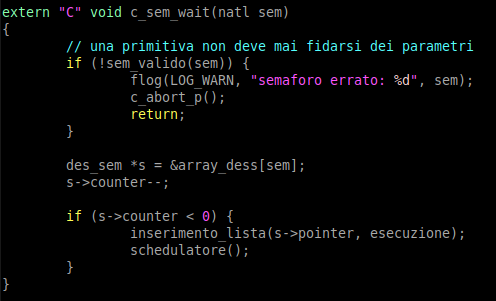
\includegraphics{img/195.PNG}\end{center} 
\begin{itemize}
	\item \underline{Eseguire questa primitiva è un po' come dire \textit{prova a prendere un gettone dal semaforo}}. 
	\item Abbiamo come unico parametro in ingresso l'identificativo del semaforo \emph{sem}.
	\item La prima cosa che facciamo è verificare la validità del semaforo utilizzando la funzione di utilità \emph{sem$\_$valido}. Nel caso in cui l'esito sia negativo si abortisce.
	\item Se l'esito della verifica è positivo si va avanti: si recupera l'indirizzo del relativo semaforo nell'array e si decrementa il contatore \emph{counter} (cioè si leva un "gettone", lo faccio SEMPRE, il valore negativo ha un significato nella primitiva \emph{sem$\_$signal}).
	\item Nel caso in cui il contatore \emph{counter} sia negativo il processo attualmente in esecuzione viene posto nella lista \emph{pointer}, successivamente viene chiamata la funzione \emph{schedulatore}.
	\item La funzione \emph{schedulatore} rimuove la testa di \emph{pronti} e ci porta ad eseguire altri processi. Il processo attuale non potrà essere eseguito finché non ci saranno "gettoni".
\end{itemize}
\subsection{Primitiva \emph{sem$\_$signal} (rilascio del gettone)}
\small 
\begin{verbatim}
	extern "C" void c_sem_signal(natl sem) {
		// una primitiva non deve mai fidarsi dei parametri
		if(!sem_valido(sem)) {
			flog(LOG_WARN, "semaforo errato: %d", sem);
			c_abort_p();
			return;
		}
		
		des_sem *s = &array_dess[sem];
		s->counter++;
		if(s->counter <= 0) {
			des_proc *lavoro = rimozione_lista(s->pointer);
			inspronti(); // preemption
			inserimento_lista(pronti, lavoro);
			schedulatore(); // preemption
		}
	}
\end{verbatim}
\normalsize  %\begin{center}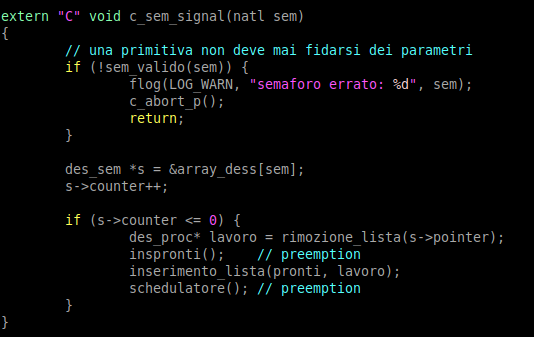
\includegraphics{img/196.PNG}\end{center} 

\begin{itemize}
	\item Abbiamo come unico parametro di ingresso l'identificativo del semaforo \emph{sem}.
	\item La prima cosa che facciamo è verificare la validità del semaforo utilizzando la funzione di utilità \emph{sem$\_$valido}. Nel caso in cui l'esito sia negativo abortisco.
	\item Se l'esito è positivo si va avanti: si recupera l'indirizzo del relativo semaforo nell'array e si  incrementa il contatore (cioè metto un "gettone", lo faccio SEMPRE).
	\item Se il contatore del semaforo è al più uguale a zero allora sono presenti processi che hanno cercato di prendere invano un gettone (e quindi sono in attesa). Quello che facciamo è estrarre uno di questi processi. \item Si ha un meccanismo di \emph{prelazione}.
	\begin{itemize}
		\item Rimuoviamo il processo dalla lista del semaforo, ci ricordiamo dove sta con una variabile temporanea.
		\item Inserisco in testa alla lista \textit{pronti} il processo attualmente in esecuzione con la funzione  \emph{inspronti} (se abbiamo lavorato bene il processo attualmente in esecuzione è quello con la priorità maggiore).
		\item Inserisco nella lista \textit{pronti} anche il processo appena estratto dalla lista del semaforo. 
		\item Chiamo  \textit{schedulatore}, l'esito sarà la scelta di uno dei due processi appena posti in \textit{pronti}.
	\end{itemize}
	\textbf{Perchè abbiamo messo il processo in esecuzione in pronti?} 
	
	Chiediamoci: cosa succede se ho processi con la stessa priorità? Ricordiamo il codice di \emph{inserimento$\_$lista}: a parità di priorità diamo un'ordinamento FIFO (chi prima arriva esce per primo). Il fatto è che inserire il processo attualmente in esecuzione in lista \emph{pronti} con \emph{inserimento$\_$lista} (e non con \emph{inspronti}) significherebbe porlo in lista dopo altri processi aventi la stessa priorità, se presenti. Con il codice scritto ci assicuriamo che il processo attualmente in esecuzione non venga sospeso se sono presenti altri processi aventi la stessa priorità: è una sottigliezza, non è sbagliato fare diversamente.
\end{itemize} 

\begin{framed}
	\noindent \textbf{Stati bloccati}.
	
	\noindent I semafori permettono l'implementazione dei cosiddetti \emph{stati bloccati}: ogni semaforo rappresenta un possibile stato bloccato, dove l'attesa dipende dal diverso significato che attribuiamo a un certo semaforo.
\end{framed} 

\begin{framed}
	\noindent \textbf{Promemoria sull'atomicità delle primitive}.
	
	\noindent Le primitive semaforiche non possono essere usate all'interno di un'altra primitiva, ne romperebbero l'atomicità. La questione sarà affrontata nel capitolo sulle periferiche, dove introdurremo delle novità.
\end{framed} 